\documentclass{article}
\title{Blanchard Ch.11}
\author{Dawei Wang}
\date{\today}
\usepackage{ctex}
\usepackage{amsmath}
\usepackage{amssymb}
\usepackage{graphicx} %插入图片的宏包
\usepackage{float} %设置图片浮动位置的宏包
\usepackage{subfigure} %插入多图时用子图显示的宏包
\begin{document}
	\maketitle

\section{产出和资本的相互作用}

长期中产出的关键性决定因素是产出与资本之间的相互作用:

资本数量决定产出数量

产出数量决定储蓄数量,由此决定累积的资本数量。

\begin{figure}[H] %H为当前位置,!htb为忽略美学标准,htbp为浮动图形
	\centering %图片居中
	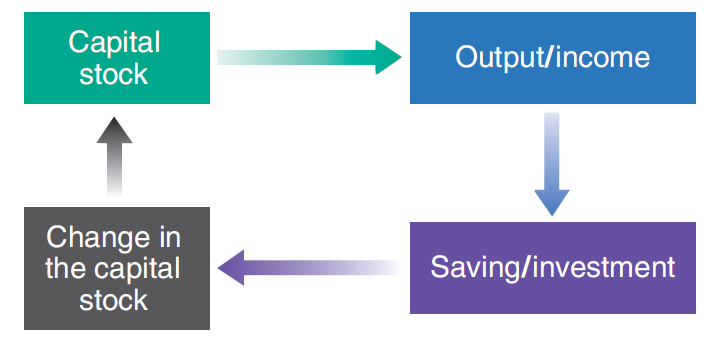
\includegraphics[width=1\textwidth]{11_1} %插入图片,[]中设置图片大小,{}中是图片文件名
	\caption{Capital, Output, and
		Saving/Investment} %最终文档中希望显示的图片标题
	\label{Fig.main2} %用于文内引用的标签
\end{figure}

\subsection{资本对产出的影响}

在规模经济不变的假设下,我们得出人均产出和人均资本的关系:

\[
\frac{Y}{N}=F(K/N,1)
\]

人均产出$ Y/N $是人均资本$ K/N $的增函数,假定资本规模递减,随着人均资本越来越多,一定量的资本增加对人均产出的影响越来越小。

将人均产出和人均资本的关系简化:

\[
\frac{Y}{N}=f(\frac{K}{N})
\]

函数f表示人均产出和人均资本的函数恒等式F等价:

\[
\frac{K}{N}\equiv F(\frac{K}{N},1)
\]

增加两个假设:

第一个假设是人口规模、参与率和失业率不变,这就意味着就业人数不变。这样单位工人的产出、人均产出和产出成比例变动。

就业人数N不变,则长期中只有资本能影响产出。

第二个假设是没有技术进步,生产函数f,也就是F函数,不会随时间变化而变化。这个假设不太符合现实,但能让我们更集中地研究资本积累的作用。

\hspace*{\fill}

有了两个假设,人均产出和人均资本的关系可以从生产的角度写成:

\[
\frac{Y_t}{N}=f(\frac{K_t}{N})
\]

总结:人均资本越高,人均产出越高。

\subsection{产出对资本积累的影响}

\subsubsection{产出与投资}

假设经济是封闭的,则

\[
I=S+(T-G)
\]

假设公共储蓄T-G为零(为研究政策对经济增长的作用,会放弃这个假设),故:

\[
I=S
\]

假设私人投资和收入(产出)成比例关系:

\[
S=sY
\]

系数s为储蓄率,取值介于0和1之间。这个假设包含两个事实:一是储蓄率不会随着该国经济的增长而自主变化;二是发达国家的储蓄率并不必然比贫困国家的储蓄率高。

引入时间变量:

\[
I_t=sY_t
\]

投资和产出成比例关系,即产出越高,储蓄越高,从而投资越多。

\subsection{投资与资本积累}

投资是流量,指一段时间内购买的及其和新修的厂房。资本是存量,指经济中某一时间存在的机器和厂房。

假设资本以每年$\delta$的速率折旧,那么从第一年到下一年,$\delta$比例的资本存量将减少。

资本存量的变化可以表示为:

\[
K_{t+1}=(1-\delta)K_t+I_t
\]

将投资与资本存量的关系式和产出和投资的关系式结合起来并求人均:

\[
\frac{K_{t+1}}{N}=(1-\delta)\frac{K_t}{N}+s\frac{Y_t}{N}
\]

变形得:

\[
\frac{K_{t+1}}{N}-\frac{K_t}{N}=s\frac{Y_t}{N}-\delta\frac{K_t}{N}
\]

简而言之,人均资本的变化量等于人均储蓄减去折旧。这个等式表示产出与资本积累的关系。

从储蓄的角度看,人均产出决定人均资本随时间的变化。

\section{不同储蓄率的含义}

\[
\frac{Y_t}{N}=f(\frac{K_t}{N})
\]

从生产的角度看,上式说明了资本如何决定产出。

\[
\frac{K_{t+1}}{N}-\frac{K_t}{N}=s\frac{Y_t}{N}-\delta\frac{K_t}{N}
\]

从储蓄的角度看,上式说明了产出如何决定资本积累。

\section{资本和产出的动态变化}

\[
\frac{K_{t+1}}{N}-\frac{K_t}{N}=sf(\frac{K_t}{N})-\delta\frac{K_t}{N}
\]

$ sf(\frac{K_t}{N}) $人均投资。本年的人均资本决定本年的人均产出,给定储蓄率的条件下,人均产出决定人均储蓄,从而决定人均投资。

$ \delta\frac{K_t}{N} $人均折旧。人均资本存量决定本年人均资本的折旧量。

如果人均投资超过人均折旧,则人均资本变化为正,即人均资本增加,反之反是。

\begin{figure}[H] %H为当前位置,!htb为忽略美学标准,htbp为浮动图形
	\centering %图片居中
	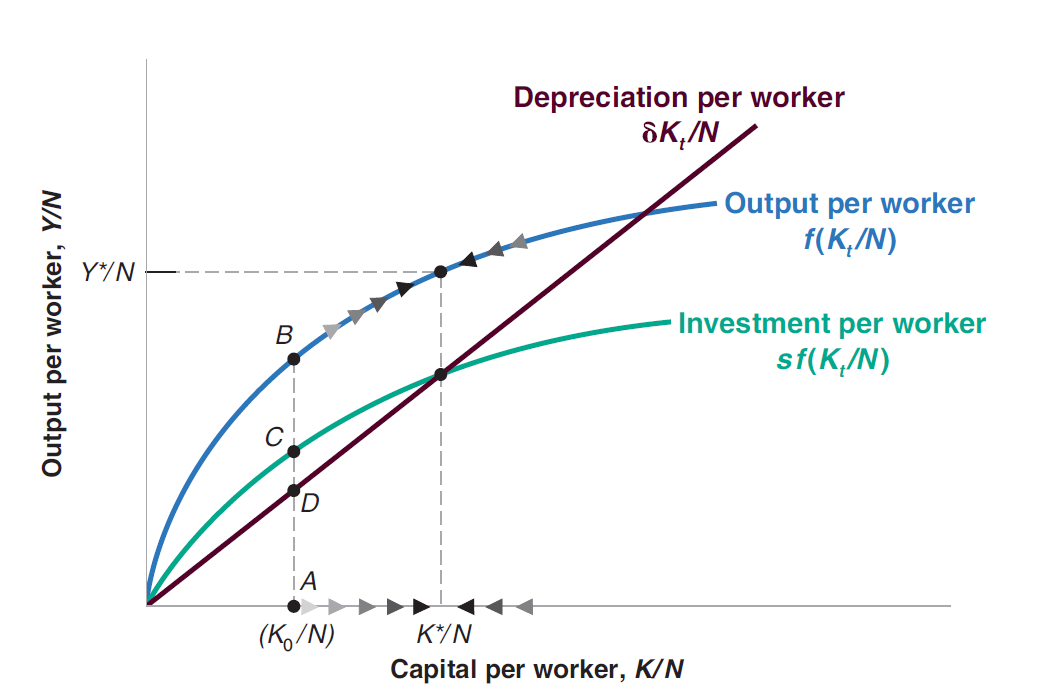
\includegraphics[width=1\textwidth]{11_2} %插入图片,[]中设置图片大小,{}中是图片文件名
	\caption{Capital and Output
		Dynamics} %最终文档中希望显示的图片标题
	\label{Fig.main3} %用于文内引用的标签
\end{figure}

人均资本的变化由人均投资和人均折旧的差额表示。人均资本较低时,人均资本和人均产出随时间增加。人均资本和人均产出随时间减少。人均资本较高时,人均资本和人均产出随时间减少。当人均资本达到$ K^*/N $处,投资等于折旧。若经济达到这一点,人均产出和人均资本都保持不变,分别为$ Y^*/N $和$ K^*/N $这就是长期均衡水平。

若一个国家在战争中遭到轰炸,资本存量减少,如果资本损失大于人口损失,那么战争会使人均资本水平较低,处于$ K^*/N $的左边。这个国家在一段时间内人均资本和人均产出都会有较大的增长。

当人均资本和人均产出不再变化时,我们称之为经济达到了稳态(steady state)。在稳态经济中,人均资本保持不变,则稳态下的人均资本$ K^*/N $可以表示为:

\[
sf(\frac{K^*}{N})=\delta\frac{K^*}{N}
\]

给定稳态下的人均资本$ K^*/N $,则稳态处的人均产出$ Y^*/N $可以由下列生产函数得出。

\[
\frac{Y^*}{N}=f(\frac{K^*}{N})
\]

\subsection{储蓄率与产出}

1. 长期中人均产出增长率为0,储蓄率不影响长期人均产出增长率。

这个结论很明显,经济最终趋向于人均产出的恒定水平。也就是说,长期不管储蓄率多大,产出增长率为0。

即使引入技术进步,在长期也不可能保持不变的正的增长率。因为如果长期保持不变的、正的增长率,人均资本必然增加。不仅如此,由于资本规模报酬递减,人均资本的增长率要大于产出的增长率。因此经济体每年需要储蓄越来越大份额的产出,并投入形成资本积累。达到某一点后,储蓄对产出的比例将会大于1,这显然是不可能的。

\hspace*{\fill}

2. 但是,储蓄率决定长期的人均产出水平。在其他条件相同时,长期中高储蓄率的国家,其人均产出水平也高。

\begin{figure}[H] %H为当前位置,!htb为忽略美学标准,htbp为浮动图形
	\centering %图片居中
	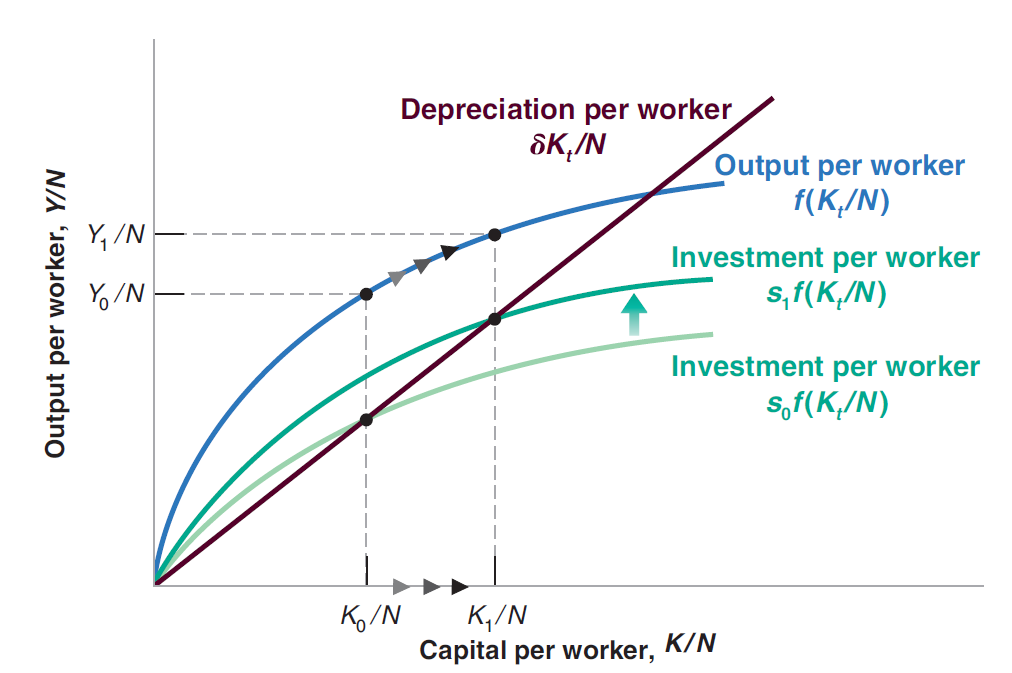
\includegraphics[width=1\textwidth]{11_3} %插入图片,[]中设置图片大小,{}中是图片文件名
	\caption{The Effects of Different
		Saving Rates} %最终文档中希望显示的图片标题
	\label{Fig.main4} %用于文内引用的标签
\end{figure}

3. 提高储蓄能在一段时间内提高人均产出,但不能一直提高。

首先,我们直到提高储蓄率并不影响长期的人均产出增长率(恒为0)。其次,提高储蓄率会提高长期的人均产出水平。由此可知,提高储蓄率导致产出达到较高的水平,经济经历了一段长时间的正增长。当经济重新回到稳态,正增长便会停止。

\begin{figure}[H] %H为当前位置,!htb为忽略美学标准,htbp为浮动图形
	\centering %图片居中
	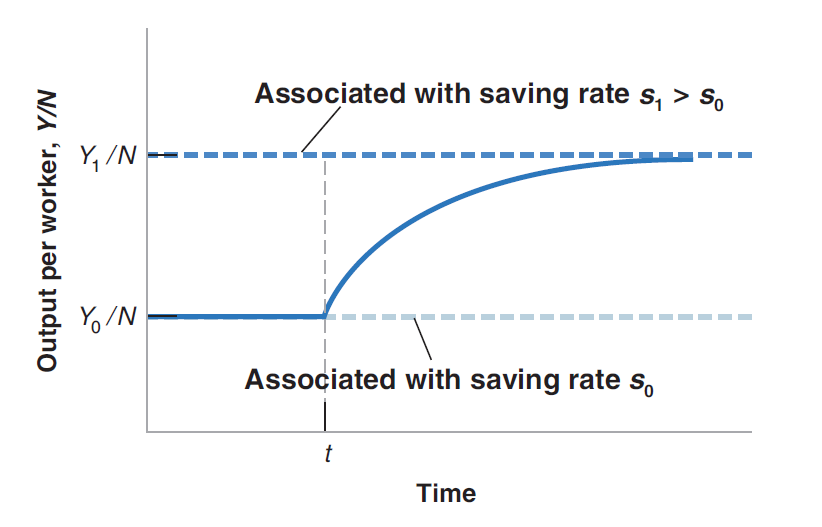
\includegraphics[width=1\textwidth]{11_4} %插入图片,[]中设置图片大小,{}中是图片文件名
	\caption{The Effects of an Increase
		in the Saving Rate on
		Output per Worker in
		an Economy without
		Technological Progress} %最终文档中希望显示的图片标题
	\label{Fig.main5} %用于文内引用的标签
\end{figure}

时间t储蓄率增加,人均产出增加,直到人均产出达到$ Y_1/N $,增长率又回到0。

\hspace*{\fill}

在没有技术进步的前提假设下,我们推导出了以上三个结论,得出长期人均产出增长率为0。

存在技术进步的情况下,一国经济即使在长期中也会出现正增长率。长期增长率与储蓄率无关,然而储蓄率影响人均产出水平。储蓄率提高后,一国经济会出现一段时间的正增长率,直到达到更高的均衡水平。

\begin{figure}[H] %H为当前位置,!htb为忽略美学标准,htbp为浮动图形
	\centering %图片居中
	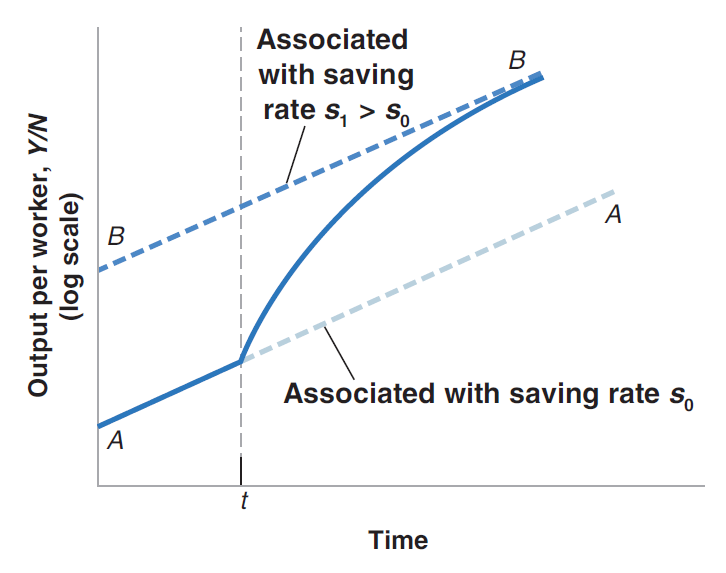
\includegraphics[width=1\textwidth]{11_5} %插入图片,[]中设置图片大小,{}中是图片文件名
	\caption{The Effects of an Increase
		in the Saving Rate on
		Output per Worker
		in an Economy with
		Technological Progress} %最终文档中希望显示的图片标题
	\label{Fig.main6} %用于文内引用的标签
\end{figure}

上图用对数来度量人均产出,因此人均产出稳定增长的经济可以用斜率等于该增长率的直线表示。储蓄率初始为$ s_0 $时,经济沿着AA线移动。在t时,储蓄率提高到$ s_1 $,经济出现一段时间正增长率,然后达到新的更高的均衡,由BB线表示。在BB线上,增长率和储蓄率提高之前的增长率一样(二者斜率相同)。


\subsection{储蓄率与消费}

政府可以通过多种途径影响储蓄。首先可以改变公共储蓄(T-G),其次政府可以改变税收来影响私人储蓄,政府对储蓄予以税收优惠,民众会更乐意储蓄,从而增加私人储蓄。

\hspace*{\fill}

从短期来说,收入一定,储蓄增加会减少消费,还可能导致经济衰退,进而收入减少。

\hspace*{\fill}

增加储蓄必然减少消费。本年的储蓄率变化不会影响本年的资本存量,也不会影响本年的产出和收入。因此,一开始储蓄增加,消费会等量减少。

长期中储蓄增加也不一定增加消费。储蓄率为0和储蓄率为1推导出的长期消费都为0。

这两种极端的情况意味着介于0和1之间的某一点的储蓄率能使经济稳态中的消费量最大。在小于该储蓄率的基础上储蓄率的增加在短期会使消费下降,但长期会增加消费。在大于该储蓄率的基础上储蓄率的增加在短期和长期都会使消费下降。因为储蓄率增加带来的资本存量增加,只会导致产出少量增加,不足以抵扣折旧部分。也就是说经济中的资本存量太高。在稳态经济中,消费水平最高时的由储蓄率所决定的资本存量称为黄金法则下的资本存量(golden-rule level of capital)。在该资本存量处再增加投资会导致消费下降。

\begin{figure}[H] %H为当前位置,!htb为忽略美学标准,htbp为浮动图形
	\centering %图片居中
	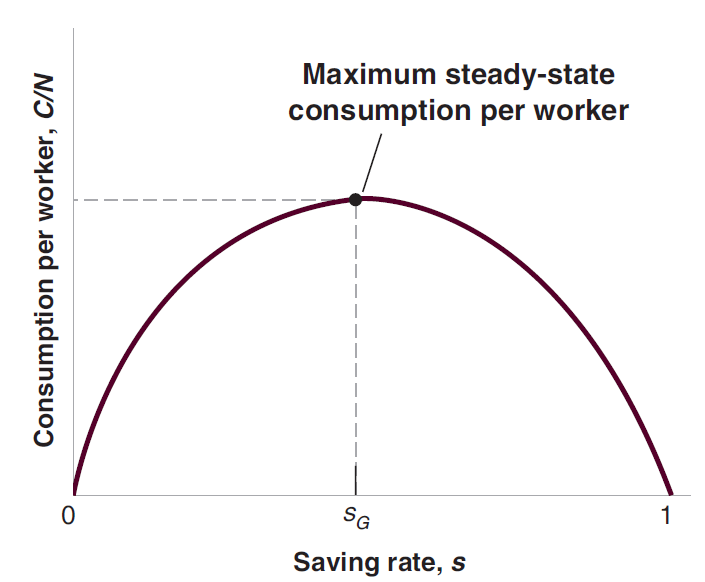
\includegraphics[width=1\textwidth]{11_6} %插入图片,[]中设置图片大小,{}中是图片文件名
	\caption{The Effects of the Saving
		Rate on Steady-State
		Consumption per Worker} %最终文档中希望显示的图片标题
	\label{Fig.main7} %用于文内引用的标签
\end{figure}

储蓄率介于0和$ s_G $之间时,储蓄率增加,人均资本增加,从而人均产出增加,人均消费增加。储蓄率大于$ s_G $时,储蓄率增加仍会增加人均产出和人均资本,但会导致人均消费减少,这是因为资本存量较大,导致较多折旧,抵消了大部分增加的产出。当$ s=1 $,人均消费为0,人均资本和人均产出很高,但所有产出用于抵扣折旧,没有用于消费。

事实上,这意味着政府需要权衡,提高储蓄率短期会减少消费,但在长期会增加消费,即提高储蓄率可能会使当代民众受损,使下一代民众受益。


\hspace*{\fill}

完全基金制社会保障系统:

用征得的税款投资金融资产,当劳动者退休的时候归还本金和利息。

私人储蓄减少,公共储蓄增加,不影响储蓄总量;

\hspace*{\fill}

现收现付制社会保障系统:

将征得的税款发放给当时退休的人员,通过征税来发放退休金。

私人储蓄减少的同时并没有增加的公共储蓄来替补,储蓄总量减少,资本存量减少。

\section{定量研究}


\section{实物资本与人力资本}

已研究的资本——机器、厂房、办公楼等属于实物资本,经济体中劳动者的技能技巧属于人力资本(human capital)。


\subsection{扩展生产函数}

修改生产函数关系式:

\[
\frac{Y}{N}=f(\frac{K}{N},\frac{H}{N})
\]

人均产出取决于实物资本量K/N,和人利资本量H/N。技能高的劳动者能从事更复杂的工作,他们能轻易解决各种突发问题,这都会提高人均产出。

人力资本规模报酬递减。

衡量人利资本的方法是按薪资对人力资本进行加权。

\subsection{人力资本、实物资本和产出}

储蓄率增加,会增加稳态下的人均实物资本和人均产出,这个结论依然成立。把这个结论扩展到人力资本,社会上人力资本形式的储蓄(通过教育和职业培训)增加,会增加稳态下的人均人力资本,从而增加人均产出。长期中,人力资本取决于社会的储蓄量和在教育上的花费。

\hspace*{\fill}

教育,尤其是高等教育,部分是为自己利益的消费支出,部分是投资。

至少就高等教育而言,人们接受教育的机会成本是放弃的收入。教育支出不仅应该包括实际的花费,还包括机会成本。

实物资本,特别是机器的折旧率高于人力资本的折旧率。人们的技能会退化,但是很慢。和实物资本不同的是,人力资本用得越多退化得越慢。

最近的研究结果认为,人力资本和实物资本在均订产出方面的作用相当。储蓄更多或者教育支出更多的国家能达到更高的稳态人均产出水平。

\subsection{内生增长}

储蓄或者教育支出更多的国家能否一直保持更高的人均产出水平?

实物资本和人力资本的共同增加可能能够维持增长。人力资本不变,实物资本增加会使规模报酬递减。实物资本不变,人力资本增加会使规模报酬递减。两者同时增加,经济能否一直持续增长?

没有技术进步而保持经济稳定增长的模型被称为内生增长模型(models of endogenous growth)。内生增长模型的增长率在长期中取决于储蓄率和教育支出比例。

\hspace*{\fill}

人均产出取决于实物资本和人力资本。两种类型的资本都可以积累——前者通过实物投资,后者通过教育和培训。提高储蓄率或者增加教育支出都能提高长期的人均产出水平,但是技术率进步不变,这些不会一直提高经济增长率。





































	
\end{document}